\chapter[O Figma]{O Figma e as motivaçoes de sua escolha como ferramenta de Prototipação.}
\label{ch:cap4}

\begin{figure}[!h]
  \centering
  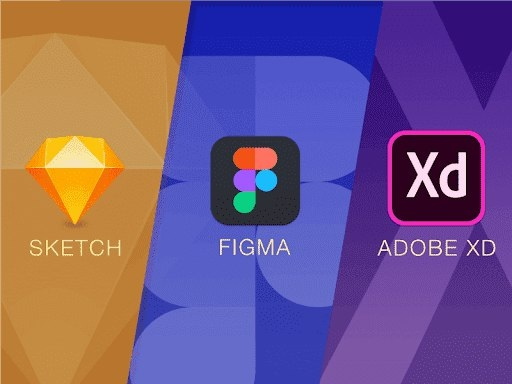
\includegraphics[width=\linewidth]{SketchFigmaAdobe.jpg}
  \caption{Figma e seus principais concorrentes.}
  \href{https://medium.com/@xccelerate/figma-vs-adobe-xd-vs-sketch-which-wireframing-tool-is-the-best-2043d458f940}{Fonte da imagem: Medium}
  \label{fig:tcenglib}
\end{figure}

Como foi dito no capitulo anterior existem diversas ferramentas de design disponiveis no mercado e os principais concorrentes são o Sketch e o AdobeXD. Ambos ferramentas muito boas e em diferentes estagios de desenvolvimento. No decorrer deste capitulo falarei mais sobre cada uma das ferramentas e explicarei os motivos que levaram a adoção do Figma para o desenvolvimento deste trabalho.

\section{Sketch} \label{Sketch}

Sketch foi desenvolvido pela Bohemian Coding e foi liberado originalmente para macOS em 2010. É considerado uma dos primeiros softwares de design de experiencia de usuario e tambem um dos primeiros softwares disruptivos no cenario UX/UI.

Como funcionalidades chaves o Sketch possui suporte a plugins assim como um preview instantanêo das alterações dos prototipos, presets de exportação automaticos de componentes, grades e linhas de guia e suporte a salvamento dos documentos em nuvem.

Algumas das vantagens do Sketch:
\begin{itemize}
  \item Desin facilmente escalável.
  \item permite a construção de bibliotecas facilitando a manutenibilidade de componentes.
  \item A funcionalidade: Pixel-perfect torna o design muito preciso.
  \item Renderização rápida e precisa em relação ao que sera mostrado no browser.
  \item Alto engajamento e suporte da comunidade.
\end{itemize}

Algumas desvantagens do Sketch:
\begin{itemize}
  \item Não possui versão gratuita.
  \item Disponivel apenas para macOS.
  \item Não possui mecanismos de edição e retoque de imagem.
  \item não possui funcionaliades de prototipação próprias dependendo de plugins.
  \item Muito dependente da comunidade em relação a manutenção de funcionalidades providas por plugins.
  \item Exigente em relação a recursos de hardware.
\end{itemize}

\section{AdobeXD} \label{AdobeXD}

O AdobeXD é a mais nova das ferramentas de design citadas neste capitulo, tendo sido lançada em 2017 pela Adobe, o software foi publicado suportando execução tanto no mac quanto no windows com extensão a testes de protototipos no ios e no android.

Possui as principais funcionalidades a co-edição, o suporte a web, desktop e mobile, drag and drop de apartir do artboard, animações automaticas e integração multi plataforma.

Algumas das vantagens do AdobeXD:
\begin{itemize}
  \item Ferramenta de design mantida pela Adobe passa a sensação de robuste e confiança.
  \item Permite a edição e o reuso de elementos com suporte a redimensionamento em grupos.
  \item Prototipos interativos com suporte a multiplas plataformas.
  \item Facilidade de uso por ususarios com experiência com outros produtos da Adobe.
  \item Salvamento em nuvem e edição de permissões de acesso como por exemplo apenas visualizar.
\end{itemize}

Algumas desvantagens do AdobeXD:
\begin{itemize}
  \item Edição de formas muito limitada, permitindo apenas formas geometricas basicas.
  \item Necessario adição de plugins para permitir visualização do CSS dos componentes.
  \item Sem suporte a edição de imagens, valendo-se do uso do Photoshop para tal.
  \item Ainda em desenvolvimento, recebe alterações constante o que pode quebrar a experiencia do uso.
  \item Apesar de gratuito durante a fase de desenvolvolvimento a Adobe pretente passar a cobrar mensalidade nos moldes de outras de suas ferramentas.
\end{itemize}

\section{Figma} \label{Figma}

O Figma foi lançado em 2016 com a proposta de ser uma ferramenta de design baseada inteiramente na nuvem. Ser um hub que permita prototipação
e desgin colaborativo. Esta mentalidade e filosofia fez com que tornase-se uma das melhores ferramentas de prototipação e design disponiveis permitindo que times trabalhem no mesmo arquivo em tempo real.

Como principais vantagens podemos destacar que é uma ferramenta totalmente baseada em nuvem, que suporta edição tanto no desktop (windows e mac) como no browser em que arquivos podem ser editados e testado tempo real pelas equipes envolvidas. Alem disso rescentemente passou a dar suporte a extensões e desenvolveu um app para android e ios chamado Figma Mirror que permite testes de prototipos usando essas plataformas mobile.

Algumas das vantagens do Figma:
\begin{itemize}
  \item Facilidade de trabalhar com grandes equipes em tempo real de forma transparente.
  \item Compartilhamento de arquivos de maneira fácil e rápida na nuvem torna os elementos de design altamente acessiveis, pulando etapas de importação e exportação.
  \item Por ser baseado em nuvem o figma se torna agnostico de plataformas.
  \item A comunidade muito ativa vem criando uma ampla variedade de plugins.
  \item Como ferramenta de prototipação e design integrados e baseado em nuvem permitindo desenvolvimento e teste colaborativo o Figma se torna um pacote completa para empresas.
  \item Possui historico de versões semelhante ao Git.
\end{itemize}

Algumas desvantagens do Figma:
\begin{itemize}
  \item Possui muito poucas funcionalidades offilne.
  \item Necessita de maquinas com desempenho intermediario para ater uma boa experiencia de uso'.
  \item A ferramenta vem recebendo constantes alterações e evoluções que podem confundir o usuário.
  \item Interface confusa.
\end{itemize}

\section{Ferramenta Adotada} \label{ferramenta_adotada}

O Figma possue serias limitações de trabalho quando a internet passa por problemas ou esta indisponivel, pois é inteiramente baseada em computação na nuvem, contudo é uma ferramenta capaz de concentrar a documentação os elementos do design e os prototipos de sistemas alem de permitir testes de usabilidade com um bom grau de fidelidade no fluxo de interações.

Além disso o figma é capaz de rodar em maquinas com desempenho intermediario, não sendo tão exigente de hardware como Sketch por exmeplo. Quanto a precifiação o Figma assim como o AdobeXD é ofertado por meio de pacotes mensais, contratados por ano ou mes a mes. contudo o figma se posiciou por manter uma serie de funcionaliades gratuitas enquanto o AdobeXD não deu garantias de mante algum pacote de serviços disponiveis como freemium. Por fim a mensalidade do Figma ainda é menor que a planejada pela Adobe para a sua ferramenta.

Por esses motivos o figma foi escolhido como ferramenta de design e prototipagem usada neste trabalho.